\chapter{Evaluation}\label{chapter:evaluation}

\section{Requirement satisfaction}

How the implementation of the stealth address scheme, as detailed in Chapter
\ref{chapter:implementation}, fulfills the functional requirements outlined in
the Chapter \ref{chapter:solution}, can be seen in Figure \ref{fig:usecase-diagram}.

\begin{figure}[h!]
    \centering
    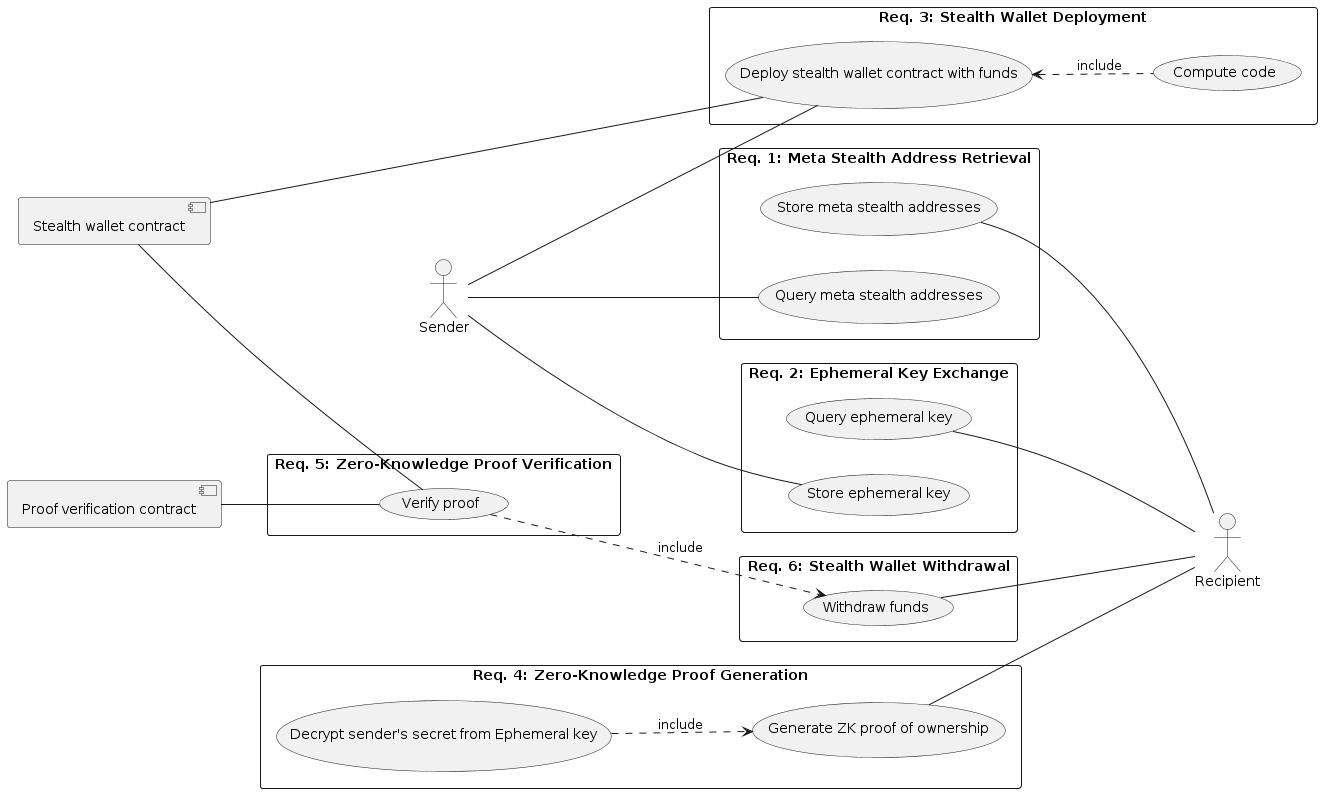
\includegraphics[width=\textwidth]{assets/images/usecase-diagram.png}
    \caption{Usecase diagram}
    \label{fig:usecase-diagram}
    \vspace{0.5cm}
\end{figure}
\pagebreak

\section{Demonstration on Sepolia Testnet}

This section walks through a demonstration of the ZKP stealth address scheme
deployed on Sepolia testnet. For this demonstration, this will be Alice's
address \href{https://sepolia.etherscan.io/address/0x2668Bc59Fa9001DBBA2bD255Bf24b9Fc8c1AbAd7}{0x2668Bc59Fa9001DBBA2bD255Bf24b9Fc8c1AbAd7}
this is Bob's primary address
\href{https://sepolia.etherscan.io/address/0x1c6Ff1028E166C9D4A15a5a019041077793c64D3}{0x1c6Ff1028E166C9D4A15a5a019041077793c64D3}
and this is Bob's second address
\href{https://sepolia.etherscan.io/address/0xc86B622175eDd2274d374dD86e13Ba521e4B876b}{0xc86B622175eDd2274d374dD86e13Ba521e4B876b}.

Both Alice's and Bob's secondary addresses have one transaction each, which were
only used to fund the address with some Ether for this demonstration.
These transactions are disregarded in this demonstration.
Bob's primary address contains one funding transaction, and two transactions
which were used to setup Bob's meta stealth address (the first transaction was
a mistake, that is why there are two). The initial state of both Alice and Bob
are shown in figure \ref{fig:alice-initial} and \ref{fig:bob-initial} respectively.

The address of the meta stealth address registry is\\
\href{https://sepolia.etherscan.io/address/0xa08aaf964300121f6c1bd962f7b53c7e06d909bd#code}{0xa08AaF964300121f6C1bD962f7B53C7e06d909BD}
and the address of the ephemeral key registry is
\href{https://sepolia.etherscan.io/address/0x156bcce17d7409a32c408e2aab8f04c8cbd7c450}{0x156Bcce17d7409A32C408e2AAb8F04C8CBd7c450}.

\begin{figure}[h!]
    \centering
    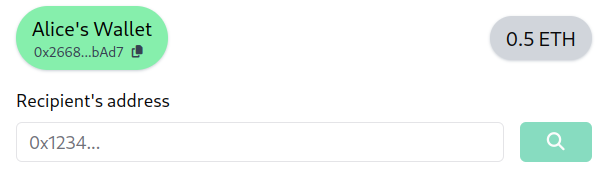
\includegraphics[width=\textwidth]{assets/images/demo/alice-initial.png}
    \caption{Initial state of Alice's wallet}
    \label{fig:alice-initial}
\end{figure}

\begin{figure}[h!]
    \centering
    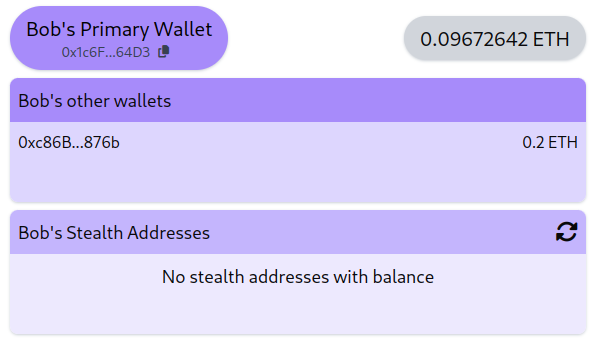
\includegraphics[width=\textwidth]{assets/images/demo/bob-initial.png}
    \caption{Initial state of Bob's wallet}
    \label{fig:bob-initial}
\end{figure}

Alice can paste Bob's primary address and query the meta stealth address
registry for his meta stealth address, shown in figure \ref{fig:meta-query}.

\begin{figure}[h!]
    \centering
    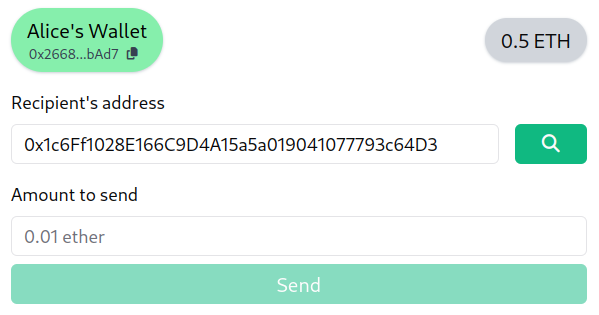
\includegraphics[width=\textwidth]{assets/images/demo/meta-query.png}
    \caption{Querying Bob's meta stealth address}
    \label{fig:meta-query}
\end{figure}

Figure \ref{fig:meta-not-found} displays scenario when Alice queries for an
address without meta stealth address.

\begin{figure}[h!]
    \centering
    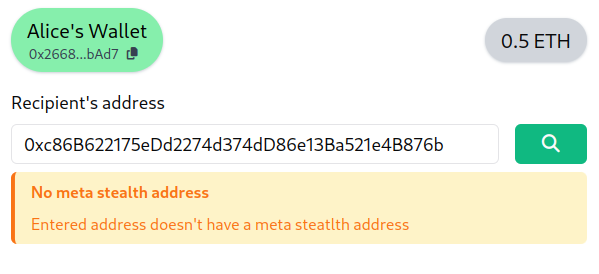
\includegraphics[width=\textwidth]{assets/images/demo/meta-not-found.png}
    \caption{Querying address without meta stealth address}
    \label{fig:meta-not-found}
\end{figure}

\pagebreak
When Alice sends funds to Bob's stealth address, she first 
\href{https://sepolia.etherscan.io/tx/0xabac631e68de9c31a4cf00d55328b9a35fff55f6baf475849197415c62b1d394}{deploys},
the stealth wallet contract and then 
\href{https://sepolia.etherscan.io/tx/0xce4a7169458a1e09ee027645c833a9a16a0ff10557a61d7fa5c3b3dabf7abee8}{submits the ephemeral key}
to the ephemeral key registry. Bob can then scan the ephemeral key registry and decrypt Alice's secret, and the
address of his stealth wallet with sent funds. Stealth wallets are then tracked,
shown in figure \ref{fig:stealth-address-tracking}.

\begin{figure}[h!]
    \centering
    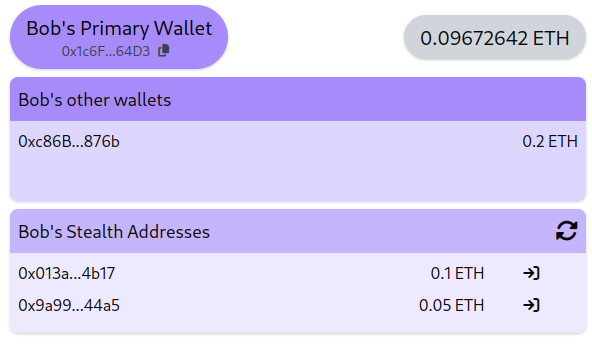
\includegraphics[width=\textwidth]{assets/images/demo/stealth-address-tracking.png}
    \caption{Tracking of Bob's stealth addresses}
    \label{fig:stealth-address-tracking}
\end{figure}

If Bob wants to use the funds, he can withdraw them to the his secondary address,
which is not linked to his primary address, as depicted in figure \ref{fig:bob-withdraw}.

\begin{figure}[h!]
    \centering
    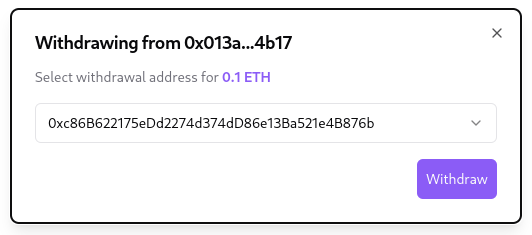
\includegraphics[width=\textwidth]{assets/images/demo/bob-withdraw.png}
    \caption{Withdrawing of funds}
    \label{fig:bob-withdraw}
\end{figure}

When accepted, the browser wallet generates a proof from Bob's secret value,
Alice's secret value and address which will be doing the withdrawal. The
proof is
\href{https://sepolia.etherscan.io/tx/0x78fabcfe3a78a7453cbe63c3f64340e80610fe6d5ceda8c250687facc52981a2}{submitted}
and funds are transferred to the chosen withdrawal address, as shown in figure \ref{fig:after-withdrawal}.

\begin{figure}[h!]
    \centering
    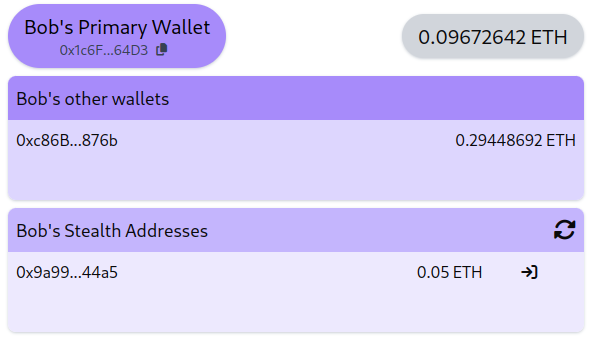
\includegraphics[width=\textwidth]{assets/images/demo/after-withdrawal.png}
    \caption{State of Bob's secondary address after withdrawal}
    \label{fig:after-withdrawal}
\end{figure}

\section{Gas analysis}

The gas consumption of the smart contracts was analyzed using the \texttt{forge test --gas-report}
command, which is part of the Foundry development framework. The most important
gas metric is the one for withdrawing funds from StealthWallet contract,
because in that function the proof validation occurs. The median for it
is \texttt{223902} gas, little higher than a Uniswap V3 swap.
The gas cost of the withdrawal function is dominated by the proof verification, which is done by
the \texttt{verifyProof} function in the \texttt{Groth16Verifier} contract. This function has a
constant gas cost of \texttt{195686}. The remaining gas is used for other operations
in the withdrawal function, such as transferring funds to the recipient.

\begin{table}[H]
    \centering
    \begin{tabular}{|l|r|r|r|r|r|}
        \hline
        \textbf{EphemeralKeyRegistry} &  &  &  &\\
        \hline
        Deployment Cost & Deployment Size &  &  &\\
        400998 & 1642 &  &  &\\
        \hline
        Function & min & avg & median & max\\
        \hline
        getKeysBatch & 423 & 4340 & 4920 & 10612\\
        submit & 58133 & 160677 & 161129 & 178229\\
        \hline
    \end{tabular}
\end{table}

\begin{table}[H]
    \centering
    \begin{tabular}{|l|r|r|r|r|r|}
        \hline
        \textbf{MetaStealthAddressRegistry} &  &  &  &\\
        \hline
        Deployment Cost & Deployment Size &  &  &\\
        501153 & 2107 &  &  &\\
        \hline
        Function & min & avg & median & max\\
        \hline
        addressMetaStealthAddress & 1956 & 3105 & 1956 & 5404\\
        setMetaStealthAddress & 25346 & 60353 & 36146 & 119051\\
        \hline
    \end{tabular}
\end{table}

\begin{table}[H]
    \centering
    \begin{tabular}{|l|r|r|r|r|r|}
        \hline
        \textbf{Groth16Verifier} &  &  &  &\\
        \hline
        Deployment Cost & Deployment Size &  &  &\\
        371621 & 1506 &  &  &\\
        \hline
        Function & min & avg & median & max\\
        \hline
        verifyProof & 195686 & 195686 & 195686 & 195686\\
        \hline
    \end{tabular}
\end{table}

\begin{table}[H]
    \centering
    \begin{tabular}{|l|r|r|r|r|r|}
        \hline
        \textbf{StealthWallet} &  &  &  &\\
        \hline
        Deployment Cost & Deployment Size &  &  &\\
        268322 & 1257 &  &  &\\
        \hline
        Function & min & avg & median & max\\
        \hline
        withdraw & 23100 & 182078 & 223902 & 257409\\
        \hline
    \end{tabular}
\end{table}

\section{Static analysis}

The implementation of the smart contracts was analyzed using the static analyzers
Aderyn \cite{githubCyfrinaderyn} and Slither \cite{githubCryticslither}.

\subsection{Aderyn results}

Static analysis of the smart contracts using the Aderyn tool revealed four low-severity issues.

\begin{enumerate}
    \item \textbf{Imprecise Solidity Pragma:} The use of a broad Solidity
        pragma \texttt{\textasciicircum0.8.13} was flagged, suggesting the use of a specific version for
        better compatibility and security. This was addressed by changing the
        pragma to pragma solidity 0.8.20;
    \item \textbf{Missing Zero Address Check:} The \texttt{StealthWallet.sol}
        lacked a check for the zero address of a verifier contract. This was
        fixed by adding the necessary check.
    \item \textbf{Public Function Optimization:} Some public functions that
        were not used internally were identified as potential candidates for being
        marked as external to optimize gas usage. These functions were modified
        accordingly.
    \item \textbf{PUSH0 Opcode Compatibility:} The report noted that the
        Solidity compiler version used could generate bytecode with PUSH0 opcodes,
        which might not be supported on all (EVM) chains.
        This was acknowledged, and it was decided to deploy the contracts only on
        chains that support EVM Shanghai, which includes the PUSH0 opcode.
\end{enumerate}

The whole report generated by Aderyn can be found in\\\texttt{stealth-wallet/aderyn-report.md}.

\subsection{Slither results}

Static analysis of the smart contracts using Slither identified several
issues, categorized as high, low, informational, and optimization.
However, it is important to note that the majority of these findings were in the
generated \texttt{Verifier.sol} contract and external library code, rather
than the core logic of the implemented stealth address scheme.

\subsubsection*{High Severity}
\begin{enumerate}
    \item \textbf{arbitrary-send-eth:} When withdrawing from stealth wallet, Ether
        could potentially be sent to an arbitrary address due to the lack of
        validation on the recipient's address in the withdraw function. This is
        not true, since only a owner can generate a valid proof, so funds
        will be transfered to address specified by the owner.
    \item \textbf{incorrect-return:} Three instances of incorrect return
        values were identified in the Groth16Verifier contract, which could halt
        execution. This contract is generated with SnarkJS, hence these issues
        can only be acknowledged. Fixing these issues in the SnarkJS generator
        is outside the scope of this project.
\end{enumerate}

\subsubsection*{Low Severity}
\begin{enumerate}
    \item \textbf{missing-zero-check: } Stealth wallet did not check if the
        recipient address is zero address, this check was added.
\end{enumerate}

\subsubsection*{Informational}
Several informational findings were related to the use of assembly code,
pragma directives, Solidity compiler versions, low-level calls, naming
conventions, and unused state variables. These were primarily found in the
generated \texttt{Verifier.sol} contract and external library code. While acknowledged,
they were not considered to directly impact the security or functionality of
the implemented scheme.

\subsubsection*{Optimization}
Two state variables in the stealth wallet contract were identified as potential
candidates for being declared as immutable, which could optimize gas usage.
These variables were made immutable.

The whole report generated by Slither can be found in\\\texttt{stealth-wallet/slither-report.md}.
